\documentclass[11pt]{article}
\usepackage[margin=1in]{geometry}
\usepackage{amsmath}
\usepackage{amssymb}
\usepackage{tikz}
\usepackage{tcolorbox}
\usetikzlibrary{patterns}
\usetikzlibrary{arrows.meta}

\title{ECO 310: Problem 2b Graphical Analysis\\WARP Violation Danger Zone}
\author{Visual Explanation}
\date{February 28, 2026}

\begin{document}

\maketitle

\section{Problem Setup}

\begin{tcolorbox}[colback=blue!5!white,colframe=blue!75!black,title=Problem 2b]
An elderly man previously consumed $(4,2)$ when prices were $(1,3)$. Prices are now $(3,5)$. Which bundles would violate WARP (get him committed)?
\end{tcolorbox}

\section{The Two Key Constraints}

For a bundle $(x_1, x_2)$ to create a WARP violation, it must satisfy BOTH:

\begin{enumerate}
\item \textbf{Inequality 1:} $x_1 + 3x_2 \leq 10$
\begin{itemize}
\item Meaning: The bundle was \textbf{affordable at old prices}
\item Old cost: $1 \cdot x_1 + 3 \cdot x_2 \leq 10$ (his original budget)
\item He could have bought this bundle before, but chose $(4,2)$ instead
\item This reveals: $(4,2) \succ (x_1, x_2)$
\end{itemize}

\item \textbf{Inequality 2:} $3x_1 + 5x_2 \geq 22$
\begin{itemize}
\item Meaning: The bundle costs \textbf{at least as much as $(4,2)$ at new prices}
\item New cost of old bundle: $3(4) + 5(2) = 22$
\item If he buys $(x_1, x_2)$ costing $\geq 22$, then $(4,2)$ was affordable
\item This reveals: $(x_1, x_2) \succ (4,2)$
\end{itemize}
\end{enumerate}

\textbf{The Contradiction:} Can't have $(4,2) \succ (x_1, x_2)$ AND $(x_1, x_2) \succ (4,2)$ simultaneously!

\newpage

\section{Visual Representation}

\begin{center}
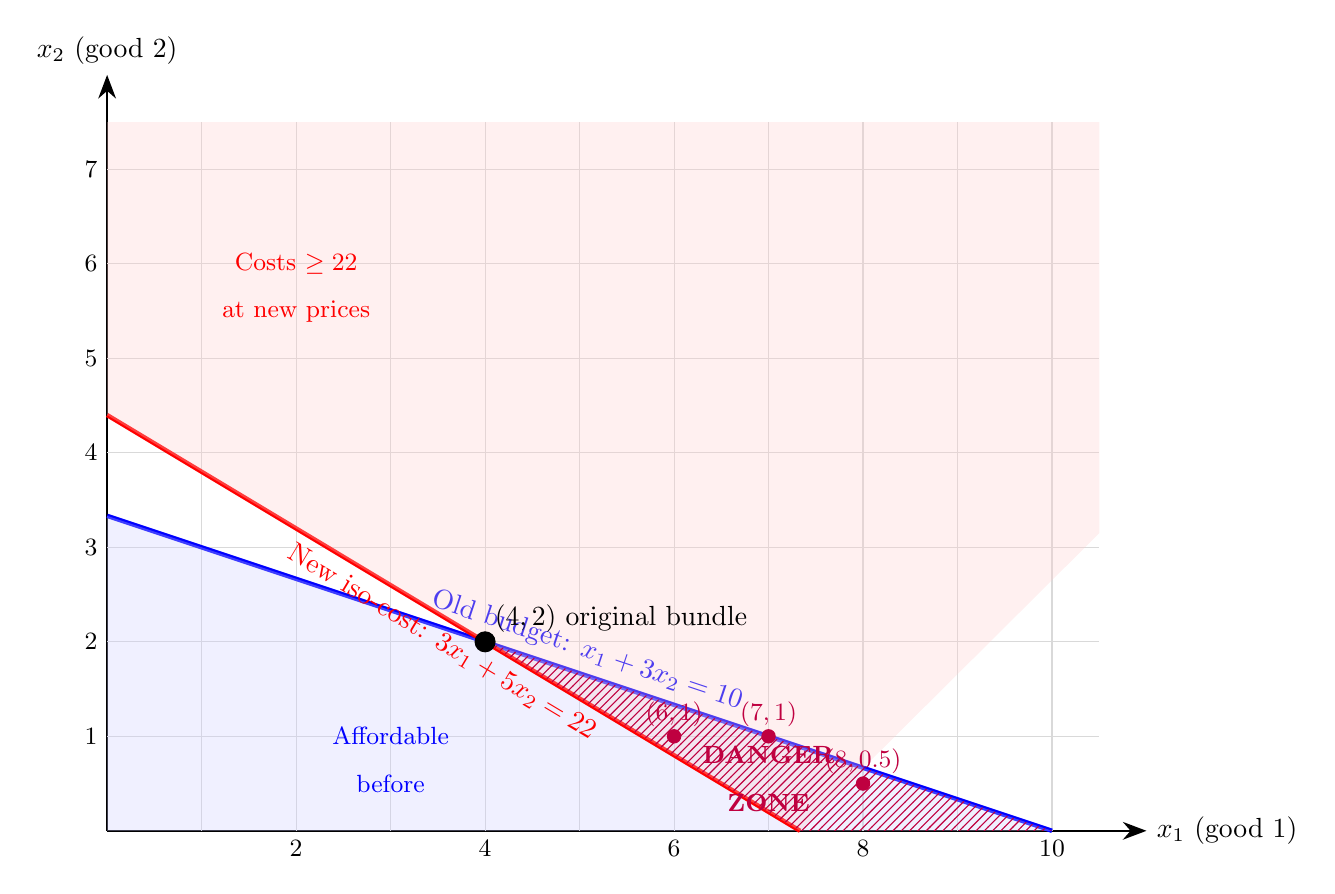
\begin{tikzpicture}[scale=1.2]
    % Draw axes
    \draw[-{Stealth[length=3mm]},thick] (0,0) -- (11,0) node[right] {$x_1$ (good 1)};
    \draw[-{Stealth[length=3mm]},thick] (0,0) -- (0,8) node[above] {$x_2$ (good 2)};

    % Grid
    \foreach \x in {1,2,...,10}
        \draw[gray!30] (\x,0) -- (\x,7.5);
    \foreach \y in {1,2,...,7}
        \draw[gray!30] (0,\y) -- (10.5,\y);

    % Old budget line: x1 + 3x2 = 10
    % When x1=0: x2=10/3≈3.33
    % When x2=0: x1=10
    \draw[blue, ultra thick] (0,3.333) -- (10,0) node[midway,above,sloped,blue] {Old budget: $x_1 + 3x_2 = 10$};

    % Fill region BELOW old budget line (was affordable)
    \fill[blue!20, opacity=0.3] (0,0) -- (0,3.333) -- (10,0) -- (10,0) -- cycle;

    % New iso-cost line through (4,2): 3x1 + 5x2 = 22
    % When x1=0: x2=22/5=4.4
    % When x2=0: x1=22/3≈7.33
    \draw[red, ultra thick] (0,4.4) -- (7.333,0) node[midway,below,sloped,red] {New iso-cost: $3x_1 + 5x_2 = 22$};

    % Fill region ABOVE new iso-cost line (costs more than old bundle)
    \fill[red!20, opacity=0.3] (0,4.4) -- (0,7.5) -- (10.5,7.5) -- (10.5,3.15) -- (7.333,0) -- (0,4.4);

    % DANGER ZONE - intersection (both blue and red)
    % Need: x1 + 3x2 ≤ 10 AND 3x1 + 5x2 ≥ 22
    % Find intersection point: solve simultaneously
    % x1 + 3x2 = 10 → x1 = 10 - 3x2
    % 3x1 + 5x2 = 22 → 3(10-3x2) + 5x2 = 22 → 30 - 9x2 + 5x2 = 22 → -4x2 = -8 → x2 = 2
    % x1 = 10 - 3(2) = 4
    % So they intersect at (4,2) - the original bundle!

    % The danger zone is actually very small/degenerate
    % Let me recalculate: the region where BOTH hold
    % Below blue line: x1 + 3x2 ≤ 10
    % Above red line: 3x1 + 5x2 ≥ 22

    % Check if there's actually a region:
    % At x2=2: blue gives x1≤4, red gives x1≥4 → only x1=4 works
    % At x2=1: blue gives x1≤7, red gives 3x1+5≥22 → x1≥17/3≈5.67
    %          So 5.67 ≤ x1 ≤ 7 works!
    % At x2=0: blue gives x1≤10, red gives x1≥22/3≈7.33
    %          So 7.33 ≤ x1 ≤ 10 works!

    % So danger zone exists below the intersection point
    % Vertices: (4,2), (10,0), (7.333,0)
    \fill[pattern=north east lines, pattern color=purple] (4,2) -- (7.333,0) -- (10,0) -- cycle;

    % Mark the original bundle (4,2)
    \filldraw[black] (4,2) circle (3pt) node[above right] {$(4,2)$ original bundle};

    % Add labels to regions
    \node[blue] at (3,1) {\small Affordable};
    \node[blue] at (3,0.5) {\small before};

    \node[red] at (2,6) {\small Costs $\geq 22$};
    \node[red] at (2,5.5) {\small at new prices};

    \node[purple, font=\bfseries] at (7,0.8) {\small DANGER};
    \node[purple, font=\bfseries] at (7,0.3) {\small ZONE};

    % Add axis labels
    \foreach \x in {2,4,6,8,10}
        \node[below] at (\x,0) {\small \x};
    \foreach \y in {1,2,3,4,5,6,7}
        \node[left] at (0,\y) {\small \y};

    % Add example points in danger zone
    \filldraw[purple] (6,1) circle (2pt) node[above] {\small $(6,1)$};
    \filldraw[purple] (7,1) circle (2pt) node[above] {\small $(7,1)$};
    \filldraw[purple] (8,0.5) circle (2pt) node[above] {\small $(8,0.5)$};

\end{tikzpicture}
\end{center}

\section{Interpretation}

\subsection{The Blue Region (Affordable Before)}

Everything below or on the blue line satisfies $x_1 + 3x_2 \leq 10$.

\textbf{What this means:} All these bundles were affordable when prices were $(1,3)$ and his budget was 10.

Since he chose $(4,2)$, he \textbf{revealed preference} that $(4,2)$ is better than any other bundle in this region.

\subsection{The Red Region (Expensive Now)}

Everything above or on the red line satisfies $3x_1 + 5x_2 \geq 22$.

\textbf{What this means:} All these bundles cost at least as much as the old bundle $(4,2)$ at the new prices $(3,5)$.

If he chooses one of these bundles now, he \textbf{reveals} he can afford at least \$22, which means $(4,2)$ is currently affordable but he's rejecting it.

\subsection{The Purple DANGER ZONE (WARP Violation)}

The crosshatched purple region is where \textbf{BOTH constraints hold}:
\begin{itemize}
\item Below the blue line (was affordable before)
\item Above the red line (costs enough now)
\end{itemize}

\textbf{Any bundle in this zone creates a logical contradiction:}

\begin{enumerate}
\item \textbf{Past behavior:} He chose $(4,2)$ over this bundle $\Rightarrow$ prefers $(4,2)$
\item \textbf{Current behavior:} He chooses this bundle over $(4,2)$ $\Rightarrow$ prefers this bundle
\item \textbf{Contradiction!} Can't prefer both A to B and B to A
\end{enumerate}

\subsection{Example Bundles That Would Get Him Committed}

\begin{itemize}
\item $(6, 1)$: Was affordable before (cost only \$9), but now costs \$23 $>$ \$22 $\times$ WARP violation
\item $(7, 1)$: Was affordable before (cost only \$10), but now costs \$26 $>$ \$22 $\times$ WARP violation
\item $(8, 0.5)$: Was affordable before (cost only \$9.5), but now costs \$26.50 $>$ \$22 $\times$ WARP violation
\item $(5, 2)$: Was NOT affordable before (cost \$11 $>$ \$10) $\checkmark$ Safe - no violation
\item $(3, 2)$: Was affordable (cost \$9) but only costs \$19 $<$ \$22 now $\checkmark$ Safe - no violation
\end{itemize}

\section{Why This Gets Him Committed}

If the elderly man purchases any bundle in the danger zone, his family can argue:

\begin{quote}
\textit{``Your Honor, our father is not of sound mind. He previously rejected bundle X when it was affordable, proving he didn't want it. But now he's buying bundle X even though his original choice is still available and affordable. This is irrational, inconsistent behavior - clear evidence he cannot make sound financial decisions.''}
\end{quote}

The court would see this as a violation of basic economic rationality (WARP), potentially supporting a claim of mental incompetence.

\subsection{The Clever Escape}

To avoid being committed, he should:
\begin{itemize}
\item Stay BELOW the red line (buy cheaper bundles that don't signal a large budget), OR
\item Stay ABOVE the blue line (buy bundles that weren't affordable before, so no revealed preference contradiction)
\item \textbf{Definitely avoid the purple danger zone!}
\end{itemize}

\end{document}
